\documentclass[11pt]{article}
\usepackage[margin=1in]{geometry}
\usepackage{amsmath, amssymb, amsthm}
\usepackage{graphicx}
\usepackage{hyperref}
\usepackage{algorithm}
\usepackage{algpseudocode}
\usepackage{tikz}
\usetikzlibrary{arrows.meta, positioning, calc}

\newtheorem{theorem}{Theorem}

\title{Mutual Information Estimation from Log-Likelihood Ratios:\\Quality Metric for Soft-Output Detectors}
\author{}
\date{}

\begin{document}

\maketitle

\section{Introduction}

In modern communication systems employing channel coding (e.g., LDPC, Turbo codes), the detector produces \textit{soft outputs} in the form of Log-Likelihood Ratios (LLRs) rather than hard bit decisions. The quality of these LLRs directly impacts the performance of the subsequent channel decoder. This document describes a practical method to evaluate LLR quality by estimating the \textbf{Mutual Information (MI)} between transmitted bits and generated LLRs.

\section{Log-Likelihood Ratios}

For a transmitted bit $b \in \{0, 1\}$, the LLR is defined as:
\begin{equation}
    L = \log \frac{P(b=0 \mid y)}{P(b=1 \mid y)}
\end{equation}
where $y$ represents the received signal (or observation). Key properties:
\begin{itemize}
    \item $L > 0$: Bit 0 is more likely
    \item $L < 0$: Bit 1 is more likely
    \item $|L|$: Confidence level (larger magnitude = higher confidence)
\end{itemize}

\section{Mutual Information as a Quality Metric}

\subsection{Definition}

The mutual information $I(X; L)$ between transmitted bits $X$ and LLRs $L$ quantifies how much information the LLRs carry about the transmitted bits:
\begin{equation}
    I(X; L) = H(L) - H(L \mid X)
\end{equation}
where:
\begin{itemize}
    \item $H(L)$: Differential entropy of the LLR distribution
    \item $H(L \mid X)$: Conditional entropy of LLRs given the transmitted bits
\end{itemize}

\subsection{Conditional Entropy Decomposition}

Assuming equiprobable bits ($P(X=0) = P(X=1) = 0.5$):
\begin{equation}
    H(L \mid X) = \frac{1}{2} H(L \mid X=0) + \frac{1}{2} H(L \mid X=1)
\end{equation}

The mutual information becomes:
\begin{equation}
    \boxed{I(X; L) = H(L) - \frac{1}{2}\left[ H(L \mid X=0) + H(L \mid X=1) \right]}
\end{equation}

\section{Information-Theoretic Foundations}

\subsection{Shannon's Channel Coding Theorem}

Claude Shannon's landmark 1948 theorem establishes the fundamental limits of reliable communication. For a discrete memoryless channel with capacity $C$:

\begin{theorem}[Channel Coding Theorem]
For any rate $R < C$, there exist codes that achieve arbitrarily small error probability. Conversely, for $R > C$, the error probability is bounded away from zero.
\end{theorem}

The channel capacity is defined as:
\begin{equation}
    C = \max_{p(x)} I(X; Y)
\end{equation}
where the maximization is over all possible input distributions $p(x)$.

\subsection{Capacity of the Binary-Input AWGN Channel}

For the binary-input additive white Gaussian noise (BI-AWGN) channel with input $X \in \{-1, +1\}$ and output $Y = X + N$ where $N \sim \mathcal{N}(0, \sigma^2)$:

\begin{equation}
    C_{\text{BI-AWGN}} = 1 - \mathbb{E}\left[ \log_2\left(1 + e^{-\frac{2Y \cdot \text{sign}(X)}{\sigma^2}}\right) \right]
\end{equation}

This can be expressed in terms of the $J$-function:
\begin{equation}
    C_{\text{BI-AWGN}} = 1 - J\left(\sigma_L\right)
\end{equation}
where $\sigma_L = \frac{2}{\sigma^2}$ is the LLR standard deviation under Gaussian assumption, and:
\begin{equation}
    J(\sigma) = 1 - \int_{-\infty}^{\infty} \frac{e^{-\frac{(l - \sigma^2/2)^2}{2\sigma^2}}}{\sqrt{2\pi\sigma^2}} \log_2(1 + e^{-l}) \, dl
\end{equation}

\subsection{The Equivalent Channel Perspective}

A key insight is that the detector creates an \textbf{equivalent channel} between the transmitted bits and the LLRs:

\begin{center}
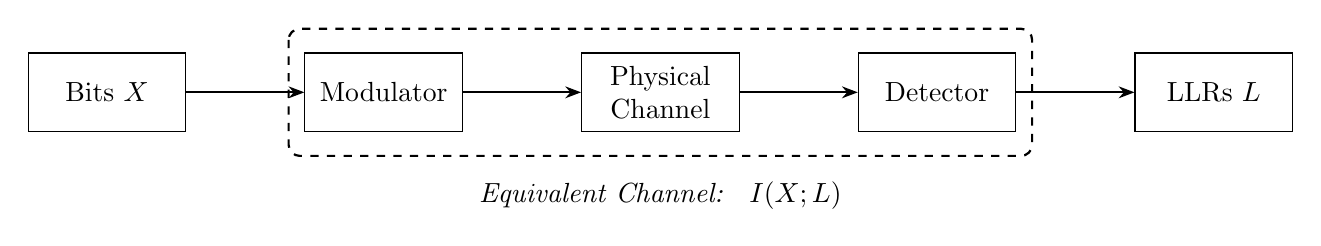
\begin{tikzpicture}[
    node distance=1.5cm,
    block/.style={rectangle, draw, minimum height=1cm, minimum width=2cm, align=center},
    arrow/.style={-{Stealth[length=2mm]}, thick}
]
    \node[block] (bits) {Bits $X$};
    \node[block, right=of bits] (mod) {Modulator};
    \node[block, right=of mod] (channel) {Physical\\Channel};
    \node[block, right=of channel] (det) {Detector};
    \node[block, right=of det] (llr) {LLRs $L$};

    \draw[arrow] (bits) -- (mod);
    \draw[arrow] (mod) -- (channel);
    \draw[arrow] (channel) -- (det);
    \draw[arrow] (det) -- (llr);

    \draw[thick, dashed, rounded corners]
        ($(mod.north west)+(-0.2,0.3)$) rectangle ($(det.south east)+(0.2,-0.3)$);
    \node[below=0.5cm of channel] {\textit{Equivalent Channel: } $I(X; L)$};
\end{tikzpicture}
\end{center}

The cascade of modulation, physical channel, and detection forms an equivalent binary-input continuous-output channel $X \to L$. The mutual information $I(X; L)$ is the \textbf{capacity of this equivalent channel}.

\subsection{Data Processing Inequality}

The data processing inequality provides a fundamental bound:
\begin{equation}
    I(X; L) \leq I(X; Y) \leq C_{\text{channel}}
\end{equation}
where $Y$ is the raw received signal. This states that:
\begin{enumerate}
    \item Processing (detection) cannot create information---only preserve or lose it
    \item The MI from LLRs is upper-bounded by the channel capacity
    \item An optimal detector achieves $I(X; L) = I(X; Y)$
\end{enumerate}

Equality holds if and only if $X \to Y \to L$ forms a \textbf{sufficient statistic}, meaning the LLRs capture all information that $Y$ contains about $X$.

\subsection{BICM Capacity}

In Bit-Interleaved Coded Modulation (BICM), each bit position in a constellation has its own equivalent channel. The BICM capacity is:
\begin{equation}
    C_{\text{BICM}} = \sum_{i=1}^{m} I(B_i; Y)
\end{equation}
where $m = \log_2 M$ is the number of bits per symbol and $B_i$ is the $i$-th bit.

For higher-order modulations (16-QAM, 64-QAM, 256-QAM):
\begin{itemize}
    \item Different bit positions have different reliabilities
    \item MSBs (Most Significant Bits) typically have higher MI than LSBs
    \item The total MI is the sum over all bit positions
\end{itemize}

\subsection{Gap to Capacity}

The \textbf{gap to capacity} quantifies detector suboptimality:
\begin{equation}
    \Delta = C_{\text{channel}} - I(X; L)
\end{equation}

\begin{itemize}
    \item $\Delta = 0$: Optimal detection (sufficient statistic preserved)
    \item $\Delta > 0$: Information loss due to suboptimal detection
\end{itemize}

For MIMO systems with interference:
\begin{equation}
    C_{\text{MIMO}} = \log_2 \det\left(\mathbf{I} + \frac{1}{\sigma^2}\mathbf{H}\mathbf{H}^H\right)
\end{equation}

The MI from LLRs measures how much of this theoretical capacity is captured by the detector.

\begin{center}
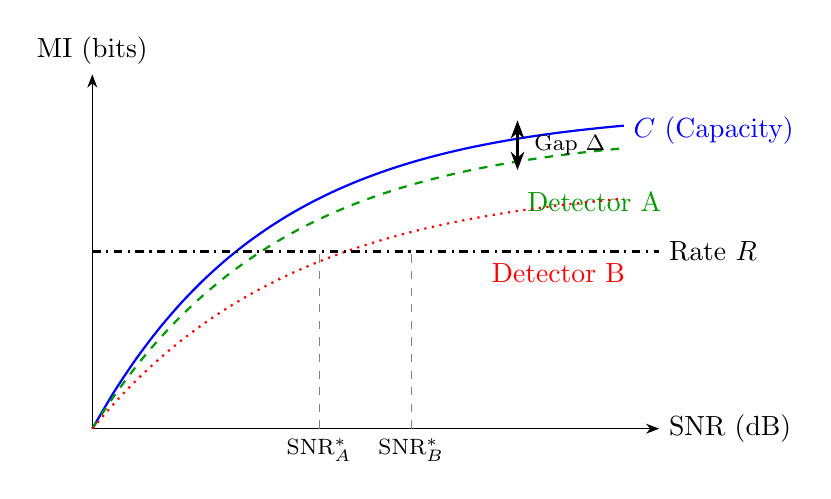
\begin{tikzpicture}[scale=0.9]
    % Axes
    \draw[-{Stealth}] (0,0) -- (8,0) node[right] {SNR (dB)};
    \draw[-{Stealth}] (0,0) -- (0,5) node[above] {MI (bits)};

    % Capacity curve
    \draw[thick, blue] plot[smooth, domain=0:7.5] (\x, {4.5*(1-exp(-0.4*\x))});
    \node[blue, right] at (7.5, 4.2) {$C$ (Capacity)};

    % Good detector
    \draw[thick, green!60!black, dashed] plot[smooth, domain=0:7.5] (\x, {4.2*(1-exp(-0.38*\x))});
    \node[green!60!black, right] at (6, 3.2) {Detector A};

    % Suboptimal detector
    \draw[thick, red, dotted] plot[smooth, domain=0:7.5] (\x, {3.5*(1-exp(-0.35*\x))});
    \node[red, right] at (5.5, 2.2) {Detector B};

    % Code rate line
    \draw[thick, black, dash dot] (0, 2.5) -- (8, 2.5);
    \node[right] at (8, 2.5) {Rate $R$};

    % Threshold points
    \draw[dashed, gray] (3.2, 0) -- (3.2, 2.5);
    \draw[dashed, gray] (4.5, 0) -- (4.5, 2.5);
    \node[below] at (3.2, 0) {\footnotesize $\text{SNR}^*_A$};
    \node[below] at (4.5, 0) {\footnotesize $\text{SNR}^*_B$};

    % Gap annotation
    \draw[{Stealth}-{Stealth}, thick] (6, 3.65) -- (6, 4.35);
    \node[right] at (6.1, 4) {\footnotesize Gap $\Delta$};
\end{tikzpicture}
\end{center}

\textbf{Interpretation}: At a code rate $R$, Detector A achieves reliable communication at $\text{SNR}^*_A$, while the suboptimal Detector B requires higher $\text{SNR}^*_B$. The gap $\Delta$ between detector MI and capacity represents lost potential.

\subsection{Consistency Condition and Optimal LLRs}

For optimal (Bayesian) LLRs, the following \textbf{consistency condition} holds:
\begin{equation}
    \mathbb{E}[L \mid X=0] = -\mathbb{E}[L \mid X=1] = \frac{\text{Var}(L \mid X)}{2}
\end{equation}

Under Gaussian assumption for the LLR distribution:
\begin{equation}
    L \mid X = x \sim \mathcal{N}\left((-1)^x \cdot \frac{\sigma_L^2}{2}, \sigma_L^2\right)
\end{equation}

This symmetry condition ensures that the LLRs are properly calibrated---the magnitude reflects the true reliability.

\subsection{Operational Meaning of MI}

The MI $I(X; L)$ has concrete operational meanings:

\begin{enumerate}
    \item \textbf{Maximum achievable rate}: With ideal coding, error-free transmission at rate $R$ bits/channel-use is possible if and only if $R < I(X; L)$.

    \item \textbf{Minimum required $E_b/N_0$}: For a target rate $R$, the minimum required energy per bit is:
    \begin{equation}
        \left(\frac{E_b}{N_0}\right)_{\min} = \frac{2^R - 1}{R} \cdot \frac{1}{\text{SNR}}
    \end{equation}
    where SNR is the signal-to-noise ratio at which $I(X; L) = R$.

    \item \textbf{Entropy reduction}: $I(X; L) = H(X) - H(X \mid L) = 1 - H(X \mid L)$ for equiprobable bits. The MI measures how much the LLRs reduce uncertainty about the transmitted bits.
\end{enumerate}

\subsection{Comparison with Uncoded Error Probability}

The relationship between MI and bit error probability $P_e$ for the BI-AWGN channel:
\begin{equation}
    I(X; L) = 1 - H_b(P_e) - D_{\text{KL}}
\end{equation}
where $H_b(p) = -p\log_2 p - (1-p)\log_2(1-p)$ is the binary entropy function and $D_{\text{KL}} \geq 0$ accounts for LLR distribution shape.

Key insight: Two systems with identical $P_e$ can have different MI values. The MI captures the \textbf{soft information quality}, not just hard decision accuracy.

\section{Implementation}

\subsection{Histogram-Based Entropy Estimation}

Since the LLR distribution is continuous, we estimate entropy using histogram binning:

\begin{algorithm}[H]
\caption{Entropy Estimation with Histogram Binning}
\begin{algorithmic}[1]
\Procedure{EntropyWithBinWidth}{$\mathbf{L}$, $\Delta$}
    \State Compute histogram with bin width $\Delta$
    \State Normalize to obtain probability density $\hat{p}(l)$
    \State $\hat{H} = -\sum_{i: \hat{p}_i > 0} \hat{p}_i \log_2 \hat{p}_i$
    \State \Return $\hat{H}$
\EndProcedure
\end{algorithmic}
\end{algorithm}

\subsection{Mutual Information Calculation}

\begin{algorithm}[H]
\caption{Mutual Information from LLRs}
\begin{algorithmic}[1]
\Procedure{CalcMI}{$\mathbf{x}$, $\mathbf{L}$}
    \State $H_L = \text{EntropyWithBinWidth}(\mathbf{L}, 0.1)$ \Comment{Marginal entropy}
    \State $\mathcal{I}_0 = \{i : x_i = 0\}$ \Comment{Indices where bit = 0}
    \State $\mathcal{I}_1 = \{i : x_i = 1\}$ \Comment{Indices where bit = 1}
    \State $H_{L|0} = \text{EntropyWithBinWidth}(\mathbf{L}[\mathcal{I}_0], 0.1)$
    \State $H_{L|1} = \text{EntropyWithBinWidth}(\mathbf{L}[\mathcal{I}_1], 0.1)$
    \State $H_{L|X} = 0.5 \cdot H_{L|0} + 0.5 \cdot H_{L|1}$
    \State $I = \max(H_L - H_{L|X}, 0)$ \Comment{Ensure non-negative}
    \State \Return $I$
\EndProcedure
\end{algorithmic}
\end{algorithm}

\section{Intuition and Interpretation}

\subsection{What Does MI Tell Us?}

\begin{enumerate}
    \item \textbf{Perfect LLRs} ($I \to 1$ bit): The LLRs perfectly predict the transmitted bits. Given the LLR value, there is no uncertainty about which bit was sent.

    \item \textbf{Useless LLRs} ($I \to 0$ bits): The LLRs carry no information about the transmitted bits. The conditional distributions $p(L|X=0)$ and $p(L|X=1)$ are identical.

    \item \textbf{Typical case} ($0 < I < 1$): Partial information is available. Higher MI indicates better-quality LLRs.
\end{enumerate}

\subsection{Visual Interpretation}

Consider the LLR distributions conditioned on the transmitted bit:
\begin{itemize}
    \item \textbf{High MI}: The distributions $p(L|X=0)$ and $p(L|X=1)$ are well-separated. LLRs for bit 0 are predominantly positive; LLRs for bit 1 are predominantly negative.

    \item \textbf{Low MI}: The distributions overlap significantly. Many LLRs have the ``wrong sign'' or are close to zero, indicating low confidence and frequent errors.
\end{itemize}

\section{Connection to Channel Coding Performance}

\subsection{Achievable Rate and Capacity}

The mutual information $I(X; L)$ represents an \textbf{achievable rate} for reliable communication:
\begin{itemize}
    \item It bounds the maximum code rate $R$ at which near-error-free transmission is possible
    \item For a capacity-achieving code (ideal LDPC at infinite block length): if $R < I(X; L)$, arbitrarily low BER is achievable
\end{itemize}

\subsection{LDPC Decoder Performance Prediction}

\begin{enumerate}
    \item \textbf{Threshold behavior}: LDPC codes exhibit a threshold phenomenon. If the MI exceeds a code-specific threshold, the decoder converges to very low error rates.

    \item \textbf{Waterfall region}: The MI directly predicts where the ``waterfall'' region of the BER curve begins. Higher MI at a given SNR means the waterfall starts at a lower SNR.

    \item \textbf{Error floor}: While MI predicts the waterfall region well, the error floor depends on code structure and is less directly tied to MI.
\end{enumerate}

\subsection{Quantitative Relationship}

For an LDPC code with rate $R$:
\begin{equation}
    \text{BER} \approx
    \begin{cases}
        \text{High} & \text{if } I(X; L) < R + \epsilon \\
        \text{Very low} & \text{if } I(X; L) > R + \epsilon
    \end{cases}
\end{equation}
where $\epsilon$ is the gap-to-capacity determined by the code design.

\subsection{Capacity-Approaching Codes and Thresholds}

Modern channel codes are designed to approach capacity:

\begin{center}
\begin{tabular}{|l|c|c|}
\hline
\textbf{Code Family} & \textbf{Gap to Capacity} & \textbf{Complexity} \\
\hline
LDPC (5G NR) & 0.1--0.3 dB & $\mathcal{O}(n)$ \\
Turbo Codes (LTE) & 0.3--0.5 dB & $\mathcal{O}(n \log n)$ \\
Polar Codes (5G control) & 0.1--0.2 dB & $\mathcal{O}(n \log n)$ \\
\hline
\end{tabular}
\end{center}

The \textbf{threshold} of a code is the minimum MI (or equivalently, minimum SNR) required for successful decoding:
\begin{equation}
    I^* = R + \epsilon_{\text{code}}
\end{equation}

For a rate-1/2 LDPC code with $\epsilon_{\text{code}} = 0.05$:
\begin{itemize}
    \item Threshold MI: $I^* = 0.55$ bits
    \item If detector provides $I(X;L) > 0.55$, near-zero BER is achievable
    \item If detector provides $I(X;L) < 0.55$, decoder will fail
\end{itemize}

\subsection{EXIT Charts and Decoding Trajectory}

EXtrinsic Information Transfer (EXIT) charts visualize iterative decoding:
\begin{itemize}
    \item \textbf{Detector curve}: Maps \textit{a priori} MI to extrinsic MI
    \item \textbf{Decoder curve}: Maps input MI to output MI
    \item \textbf{Tunnel}: Decoding succeeds if curves don't intersect
\end{itemize}

The initial MI $I(X; L)$ from the detector determines the starting point. Higher initial MI opens a wider decoding tunnel, enabling convergence at lower SNR.

\section{Practical Implications}

\subsection{Detector Comparison}

MI enables fair comparison of different detection algorithms:
\begin{itemize}
    \item Compare LMMSE, neural network detectors (ESCNN), sphere decoding, etc.
    \item A detector with higher MI will yield better coded BER, even if uncoded BER is similar
\end{itemize}

\subsection{LLR Calibration}

Poorly calibrated LLRs (e.g., over-confident or under-confident) reduce MI:
\begin{itemize}
    \item \textbf{Over-confident}: LLR magnitudes too large $\to$ decoder trusts wrong bits too much
    \item \textbf{Under-confident}: LLR magnitudes too small $\to$ decoder ignores reliable information
\end{itemize}

The MI metric captures these calibration issues, making it more informative than hard-decision BER for coded systems.

\subsection{Why MI Matters More Than Uncoded BER}

\begin{center}
\begin{tabular}{|l|c|c|}
\hline
\textbf{Scenario} & \textbf{Uncoded BER} & \textbf{MI} \\
\hline
Detector A & 5\% & 0.70 bits \\
Detector B & 5\% & 0.85 bits \\
\hline
\end{tabular}
\end{center}

Both detectors have identical uncoded BER, but Detector B provides better LLRs. After LDPC decoding:
\begin{itemize}
    \item Detector A: Coded BER $\approx 10^{-3}$
    \item Detector B: Coded BER $\approx 10^{-6}$
\end{itemize}

\section{Summary}

The mutual information between transmitted bits and LLRs:
\begin{enumerate}
    \item Measures the \textbf{information content} of soft outputs
    \item Predicts \textbf{channel coding performance} (LDPC, Turbo, Polar codes)
    \item Captures \textbf{LLR quality} beyond simple error counting
    \item Enables \textbf{fair comparison} of detection algorithms for coded systems
    \item Represents the \textbf{capacity of the equivalent channel} formed by the detector
    \item Is bounded by the \textbf{channel capacity} via the data processing inequality
\end{enumerate}

The implementation uses histogram-based entropy estimation with the formula:
\begin{equation}
    I(X; L) = H(L) - \frac{1}{2}\left[ H(L \mid X=0) + H(L \mid X=1) \right]
\end{equation}

Higher MI indicates that the detector produces LLRs that will lead to better performance when paired with a channel decoder such as LDPC.

\subsection{Key Information-Theoretic Insights}

\begin{enumerate}
    \item \textbf{Shannon's theorem}: Reliable communication is possible at rates below MI, impossible above.

    \item \textbf{Data processing inequality}: Detection cannot create information---$I(X;L) \leq I(X;Y) \leq C$.

    \item \textbf{Equivalent channel}: The detector creates a binary-input soft-output channel whose capacity equals the measured MI.

    \item \textbf{Threshold behavior}: Capacity-approaching codes (LDPC, Polar) exhibit sharp thresholds---decoding succeeds when $I(X;L) > R + \epsilon$, fails otherwise.

    \item \textbf{Soft information matters}: Two detectors with identical BER can have vastly different MI, leading to different coded performance.
\end{enumerate}

\section*{References}

\begin{enumerate}
    \item C. E. Shannon, ``A Mathematical Theory of Communication,'' \textit{Bell System Technical Journal}, vol. 27, pp. 379--423, 1948.

    \item G. Caire, G. Taricco, and E. Biglieri, ``Bit-Interleaved Coded Modulation,'' \textit{IEEE Trans. Inf. Theory}, vol. 44, no. 3, pp. 927--946, May 1998.

    \item S. ten Brink, ``Convergence Behavior of Iteratively Decoded Parallel Concatenated Codes,'' \textit{IEEE Trans. Commun.}, vol. 49, no. 10, pp. 1727--1737, Oct. 2001.

    \item T. Richardson and R. Urbanke, \textit{Modern Coding Theory}, Cambridge University Press, 2008.

    \item F. Brännström, L. K. Rasmussen, and A. J. Grant, ``Convergence Analysis and Optimal Scheduling for Multiple Concatenated Codes,'' \textit{IEEE Trans. Inf. Theory}, vol. 51, no. 9, pp. 3354--3364, Sept. 2005.
\end{enumerate}

\end{document}
